\section{Implementation and evaluation of the object detector}

In this section I will describe the YOLOv3 structure of the convolutional neural network used to train the synthetic model $\mathcal{S}$ and the hand labeled model $\mathcal{H}$.
The datasets used are described and the training parameters for each of the models are explained.
Finally I will explain the method of comparing the two models and discuss the results.

\subsection{YOLOv3 model}
The neural network structure as introduced in \cite{redmon2018yolov3} used for feature extraction is called \textit{Darknet-53} and shown in Figure \ref{fig:darknet}.
The network is a fully connected convolutional network and has 75 convolutional layers overall.
The network consists of multiple blocks marked by boxes in Figure \ref{fig:darknet}.
Each block has an additional shortcut connection, similar to skip connections used in ResNet, around it.
The blocks consist of two successive convolutional layers with kernel size $3$ and kernel size $1$ followed by a $Residual$ layer.
In between each block a convolutional layer with stride 2 is used to downsample the feature maps.
Also no pooling is used to prevent the loss of low-level features.
Lastly global average pooling is applied.
The output layer is a fully connected layer with 1000 nodes followed by a softmax activation function.

Each unit in the resulting feature map can predict up to 3 bounding boxes.
A bounding box consists of the box's center coordinates, its width, height, the objectness score and the class confidence.
The network predicts 4 coordinates for each bounding box: $t_x, t_y, t_w, t_h$.
Together with the bounding box offset within the image $c_x, c_y$ and the box prior $p_w, p_h$ the bounding box center coordinates and dimensions are computed as
\begin{equation}
\begin{split}
b_x = \sigma(t_x) + c_x\\
b_y = \sigma(t_y) + c_y\\
b_w = p_we^{t_w}\\
b_h = p_he^{t_h}\\
\end{split}
\end{equation}
During the training the loss is computed as the sum of squared errors.

More details on the prediction of the bounding boxes, the objectness score and the class confidences can be found in \cite{redmon2018yolov3}.

\begin{figure}
\centering
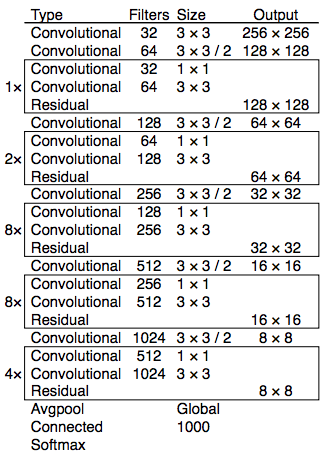
\includegraphics[width=0.4\textwidth]{figures/yolov3.png}
\caption{Structure of the YOLOv3 Darknet-53 neural network \cite{redmon2018yolov3}.}
\label{fig:darknet}
\end{figure}

\subsection{The training data}
Information about the training datasets can be seen in Table \ref{tab:1}.
The synthetic dataset consisted of 6200 automatically generated imagtes with different parameter variations.
All images were in JPEG format with their corresponding labels being txt files in the format:\\
\textit{<object class> <x center> <y center> <width> <height>}.

The old dataset consisting of 481 images was annotated using the tool \href{https://github.com/tzutalin/labelImg}{LabelImg}.
The tool generate xml labels with a different format, thus I wrote a script to convert the xml labels to the above format.

The difference between the two datasets is that the synthetic data can distinguish the different types of minions and therefore has 5 detectable object classes instead of 3.
The following classes are included in the synthetic dataset:
\begin{itemize}
\item Red side towers
\item Red melee minion
\item Red caster minion
\item Red canon minion
\item Champion Vayne (red skin, because back then when I labeled the old dataset I thought this would somehow to contrast from the background, but I also made a synthetic dataset with the default skin)
\end{itemize}
In the hand labeled dataset the minions are grouped into one class.

In case one wants to train the synthetic model with only three classes, combining the minions into one class, I wrote a script that can do so by replacing object class IDs: (\texttt{rename\_classes.py}).

\subsection{Training the models}
The models have been trained using \textit{darknet}~\cite{darknet13}\footnote{\href{https://pjreddie.com/darknet/}{Darknet Website}, \href{https://github.com/pjreddie/darknet}{GitHub}}, an open source neural network framework written in C.
I selected this method because it was easy to setup and run on GPUs. Since I implemented the network and the detection code myself I could have written a training script myself, but for saving time on this already huge project I resorted to use this implementation.

Note that the new model trained on the synthetic dataset is additionally capable of differentiating the 3 different minions classes instead of grouping them as just enemies.
Therefore, $\mathcal{S}$ is capable of detecting 5 classes compared to $\mathcal{H}$ which can only detect 3.
This means of course that we require more data to train $\mathcal{S}$ and a longer time to train.

\subsubsection{Training on hand labeled data}
The parameters used when training $\mathcal{S}$ can be seen in Table \ref{tab:1}.
The model was trained on one Nvidia 1080Ti GPU with a batch size of 64. The image width differed, because the old labeled training data I had was on images with a resolution or 1280x1024 compared to the new images with 1920x1080.
However, this should not be a problem since the network used is a fully connected convolutional network and the input size of the images does not matter as long as it stays constant.
The angle parameter sets the maximum random rotation of the images while training.
Since the objects to train are already rotated in the dataset generation and the game is always played from the same perspective, this is not necessary.
The Saturation, Exposure and Hue values set the random values for further random image manipulation.
The values use are the standard values.
The learning rate was also left at standard values.
The burn-in episodes were set to 500.
The burn in time is the number of episodes in the beginning of the training during which the learning rate will grow from 0 to its intended value.
I have read online that this has been found to increase the training speed, but I have not found any papers that show that and I have been able to verify this myself.
The model was trained for 7500 episodes, because the relatively low size of the training dataset could lead to overfitting if more episodes were used.

\subsubsection{Training on synthetic data}
\begin{figure}[t]
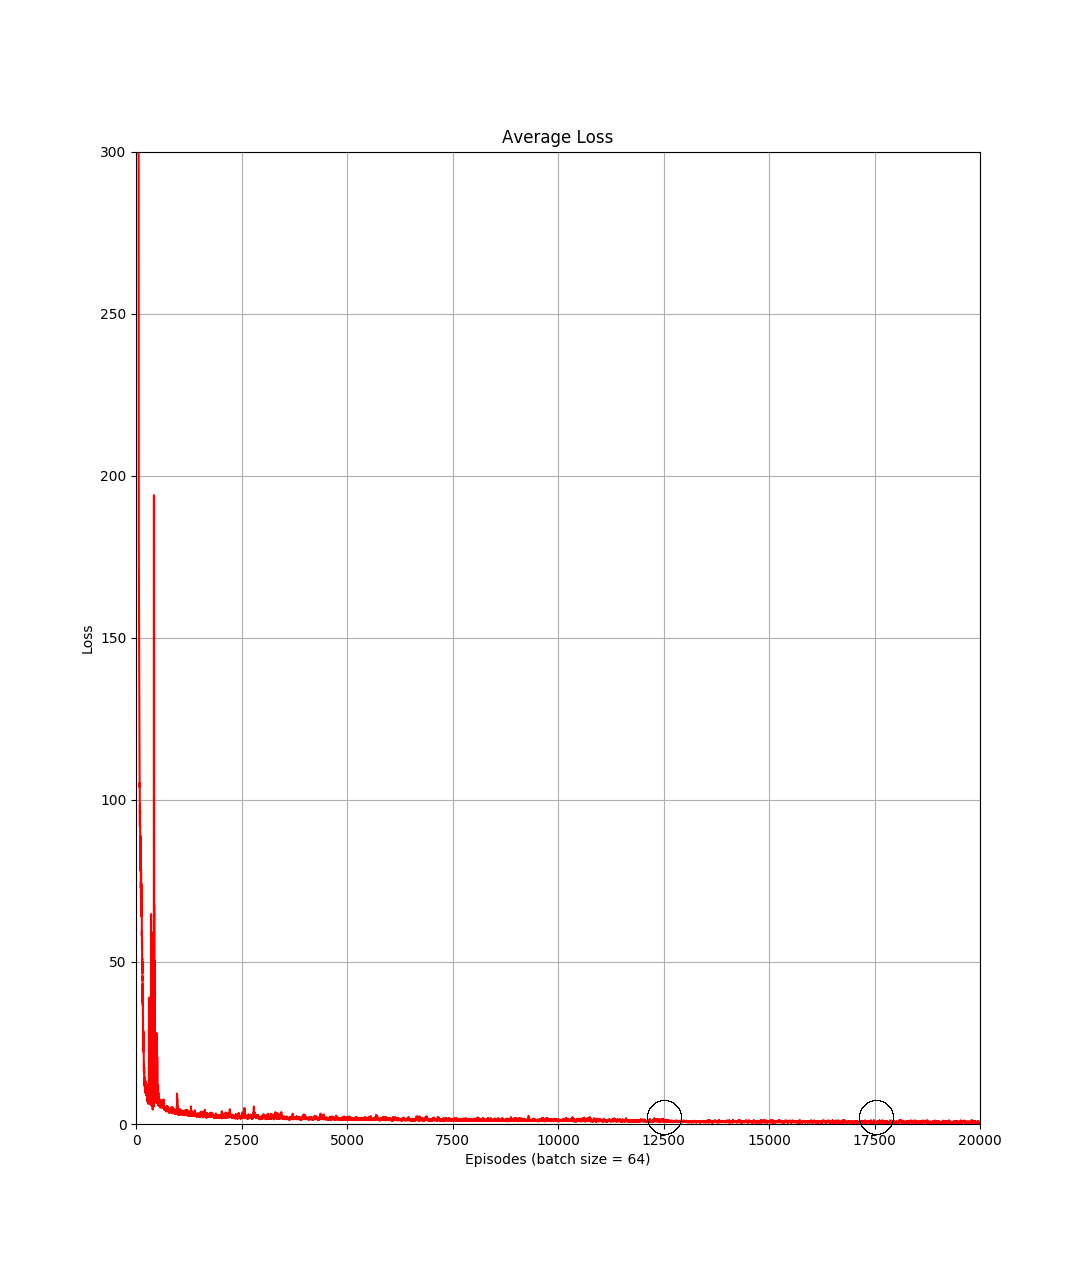
\includegraphics[width=0.5\textwidth]{figures/loss.png}
\caption{Loss per episode during training of the model with the synthetic dataset. Training for 40000 episodes with batch size 64 on two Nvidia 1080Ti GPUs. The scale is only until 20000 episodes, because when using two GPUs darknet halfs the number of episodes.}
\label{fig:loss}
\end{figure}
\begin{table*}[h]
\centering
\caption{Training config parameters for synthetic dataset $\mathcal{S}$ and hand labeled dataset $\mathcal{H}$.}
\label{tab:1}
\begin{tabular}{|l|ccc|}
\hline
	Model 			& $\mathcal{S}$ & $\mathcal{H}$ & $\mathcal{C}$\\
\hline
	Number of images& $6200$		& $481$	& $6681$\\
	Image resolution& $1920 \times 1080$	& $1280 \times 1024$ & $1920 \times 1080 $ and $1280 \times 1024$ \\
	Classes			& $5$			& $3$ & 3 \\
	Dataset creation time & 30 min & 24 hours & -\\
\hline
	Batch size		& $64$			& $64$  & $64$ \\
	Image width 	& $960$ 		& $640$	& $960, 640$\\
	Angle			& $0$ 			& $0$ 	& $0$\\ 
	Saturation		& $1.5$ 		& $1.5$ & $1.5$ \\
	Exposure		& $1.5$ 		& $1.5$ & $1.5$ \\
	Hue				& $0.1$ 		& $0.1$ & $0.1$ \\
\hline
	Learning Rate	& $0.001$ 		& $0.001$ & $0.001$	\\
	Burn In	Episodes &$1000$		& $500$   & $1000$	\\
	Max. Episodes	& $40000$ 		& $7500$  & $40000$	\\
	Reduce LR at	& $25000, 35000$& $5000$  & $25000, 35000$	\\
	Reduce LR by	& $0.1, 0.1$ 	& $0.1$	 & $0.1, 0.1$	\\
\hline
	Training time   & $70$ hours (2 GPUs) & $12$ hours (1 GPU) & $70$ hours (2 GPUs) \\
\hline
\end{tabular}
\end{table*}

The parameters for the synthetic data can be seen in Table \ref{tab:1}.
The batch size of 64 was effectively twice as large as for training $\mathcal{H}$ because the training ran on 2 GPUs. Therefore the plot in Figure \ref{fig:loss} is from $0$ to $20000$ with different learning rate reduction values.
Similar to the training of $\mathcal{H}$, the angle, saturation, exposure and hue values are unchanged.
The training loss on the synthetic dataset is shown in Figure \ref{fig:loss}.
It can be seen that the loss declined quite rapidly in the first 2500 episodes.
However, when testing models trained for less than 10000 episodes, the mAP of $\mathcal{S}$ was significantly lower than the mAP of $\mathcal{H}$ trained with only 7500 episodes.
This is a result of the fact that $\mathcal{S}$ was trained with more images and with more different classes.
The learning rate for $\mathcal{S}$ was the same as the standard value used for existing YOLOv3 models.
The burn-in rate here was selected larger because more maximum episodes were used.
Furthermore the reduction of the learning rate (marked as black circles), helped the learning process of $\mathcal{S}$ as can be seen from the decrease of the loss around 25000 episodes.
The reduced learning rate was introduced to prevent overfitting of the model.



\subsection{Comparing the datasets}
\begin{table*}
\centering
\caption{Mean average precision on the test set per class and model. Tracking of the player character in percent of the whole video.}
\label{tab:2}
\begin{tabular}{|l|ccc|}
\hline
	Model 			& $\mathcal{S}$ & $\mathcal{H}$ & $\mathcal{C}$ \\
\hline
	Input resolution& $640 \times 360$ & $640 \times 524$ & $960 \times 540$\\
\hline
	mAP Tower		& $0.81$	& $0.5$  & $0.75$ \\
	mAP All minions & $0.85$ (weighted average)	& $0.83$ & $0.83$ \\
	mAP Canon		& $1.0$		&		 & \\
	mAP	Caster		& $0.93$	& 		 & \\
	mAP Melee		& $0.73$	&		 &\\
	mAP Vayne		& $1.0$		& $0.81$	& $0.94$\\
\hline
	Character tracking time in percent of the whole video: & & &\\
\hline
	Correctly detected character & $88.53\%$ & $84.12\%$ & $73.2\%$ \\
	Detected character multiple times & $8.87\%$ & $0.28\%$ & $1.73\%$ \\
	No detection 	& $2.6\%$ & $15.6\%$ & $25.1\%$\\
	FPS	on a GTX1080		& $18$		& $12$ & $10$\\
\hline
\end{tabular}
\end{table*}
In order to compare the models, I created a hand labeled test set of 54 images.
On this test set I computed the mean average precision (mAP) as defined in the \href{http://host.robots.ox.ac.uk/pascal/VOC/voc2012/}{PASCAL VOC 2012 competition (Link)} using the script \texttt{LeagueAI\_mAP.py}.
The mAP is computed as the number of correct classifications of an object (true positives) by the number of occurences in the dataset.
An object counts as correctly classified if their Intersections divided by their union area \textit{IoU} >= 0.5.
The computation of the IoU of an object is visualized in Figure \ref{fig:iou}.
\begin{figure}[h]
\centering
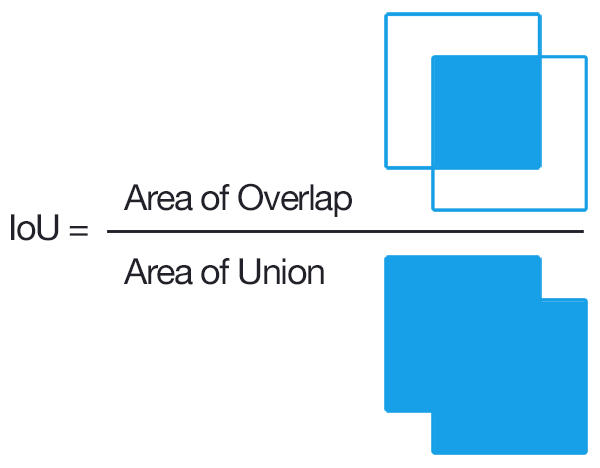
\includegraphics[width=0.2\textwidth]{figures/iou_equation.png}
\caption{Computation of the Intersection to Union ratio. Image from \href{https://www.pyimagesearch.com/wp-content/uploads/2016/09/iou_equation.png}{Link}.}
\label{fig:iou}
\end{figure}
For each object class $I$ I counted the correct ($IoU >= 0.5$), wrong (different class or $IoU < 0.5$) and not detected ground truth labels and divided them by the total number of class occurrences in the dataset $T$.

\begin{equation}
mAP = \frac{1}{T} \sum^{I}_{i=0} 1~|~\{IoU_i >= 0.5\}
\end{equation}

To evaluate the performance of both model in a real-time environment I used the video from which the hand labeled test dataset was generated.
The 126 seconds video clip was recorded in a normal game setting and includes tests such as zooming in, using abilities and attack minions.
In order to play the game it is crucial to know the location of one's player character.
Therefore I computed how long each model was able to detect the player character.

\subsection{Results}
The results of both models on the test set are shown in Figure \ref{fig:results_old} for $\mathcal{H}$ and \ref{fig:results_new} for $\mathcal{S}$.
Table \ref{tab:2} shows the numerical results from comaring the mAP of all three models on a hand labeled test dataset and a video.
The combined dataset $\mathcal{C}$ will be discussed later as there might have been problems with the training and the results do not allow for an accurate comparison.

Also important to note is that the comparison is in favor of the hand labeled model, since it only has to differentiate between 3 classes while the synthetic model is also capable of telling apart the different types of minions.
The champion Vayne and the Tower class however are directly comparable.
Furthermore, testing showed that while mode $\mathcal{S}$ was trained on higher resolution data, it performed better for lower resolution input images leading to a higher mAP and more frames per second processed.
The same effect could not be confirmed on the hand labeled data.
The input resolution of the test data is shown in Table \ref{tab:2}.
Due to the lager dataset and more object classes, training model $\mathcal{S}$ took much longer at 70 hours on two Nvidia GTX 1080Ti GPUs compared to 12 hours on one GPU for model $\mathcal{H}$.

The results of the mAP on the test dataset showed that in the test set most of the objects were minions (which is usually in the game the case since they appear in groups of 6-7).
Also the canon minion type is more rare.
Furthermore, we can see that most wrong detections happened among the melee and caster minions.
This is because they usually move in groups of 3 each and overlap each other during fighting.
The worst performance was recorded for the melee minion, resulting from the overlapping with another additional group of minions currently not detected by the model: the melee minions of the player's team.

Comparing the mAP on the hand labeled test dataset shows that model $\mathcal{S}$ provides a higher mean average precision across all classes while at the same time being able to discern more classes.
The relatively low performance of both models on the tower, a static object, is most likely a result of the size of the tower.
Compared to the other game objects it is larger and therefore most of the time only partially on the screen and often overlapped by other objects.
The findings in this report do not confirm the findings in \cite{rajpura2017object}, that the synthetic data leads to less precise object detection.
However, the 2D nature of the data generation on a video game with a limited number of objects and animation phases is not as complex as a 3D environments.
Especially considering that video games are usually designed in a way that the objects are easily discernible by the human players and therefore probably also for an object detector.

To evaluate the performance in a real-time scenario, I used the video from which the 54 test images were extracted and computed the average tracking times of the player character.
The results are listed in Table \ref{tab:2}.
It can be seen that both models could track the player character more than $84\%$ of the time where mode $\mathcal{S}$ has a slight advantage with $88.5\%$.
\begin{figure}[H]
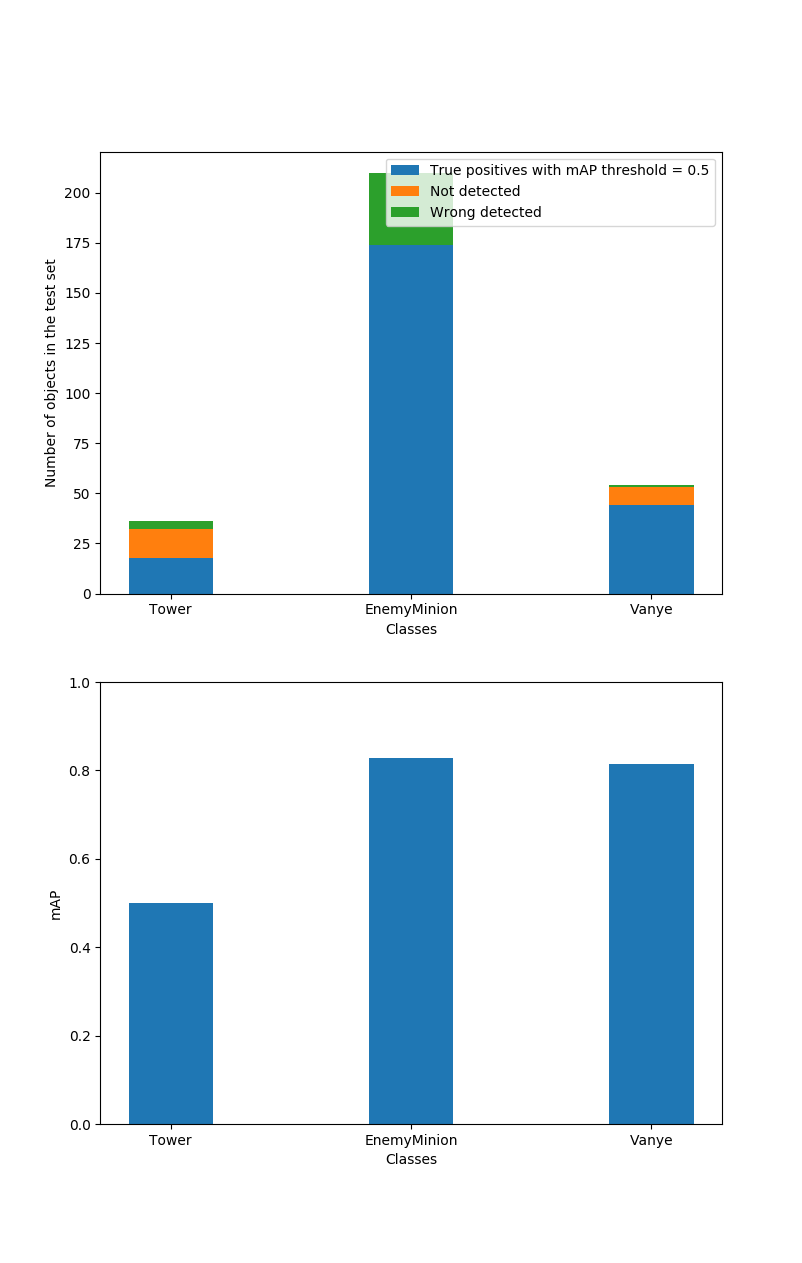
\includegraphics[width=0.5\textwidth]{figures/old.png}
\caption{Mean average detection precision per class on a test set of 54 hand labeled images for the old model tained on hand labeled data.}
\label{fig:results_old}
\end{figure}

Interestingly, model $\mathcal{H}$ was 7 times more likely to not detect the character than $\mathcal{S}$.
On the other hand $\mathcal{S}$ 40 times more likely to detect the player character and other objects that were mistaken for the player character.
However, multiple detections are not as big of a problem as losing tracking entirely since sorting the list of possible character detections by their confidence usually gives the correct object as the detection with the highest confidence.
\begin{figure}[H]
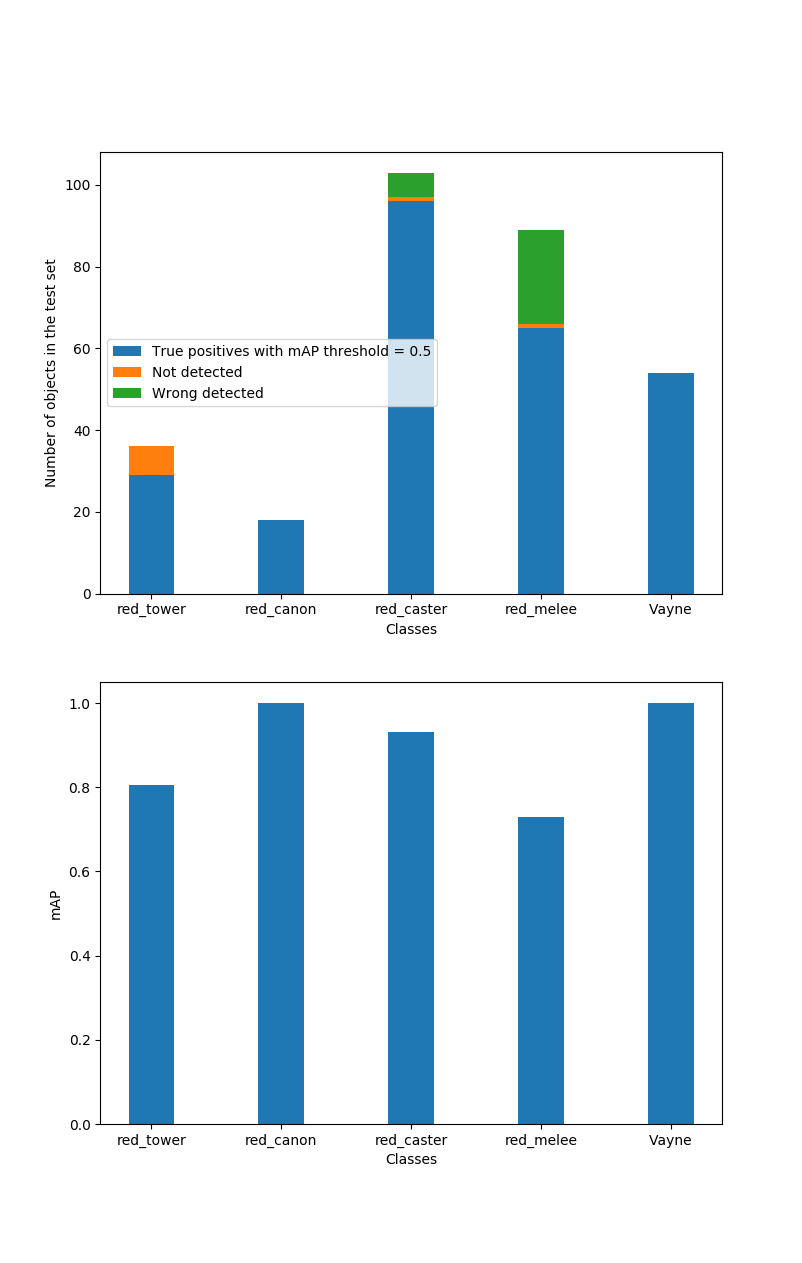
\includegraphics[width=0.5\textwidth]{figures/new_05_02_final.png}
\caption{Mean average detection precision per class on a test set of 54 hand labeled images for the new model trained on synthetic data. Note that here the minion category is split up in the three different types of minions.}
\label{fig:results_new}
\end{figure}
Also noteworthy is that as a result of the lower image resolution, the average FPS using model $\mathcal{S}$ was 50\% higher.
Therefore we can conclude that in a real time scenario the synthetic data leads to a more precise model than hand labeled data.

Lastly I will analyze three specific cases from the 54 test images that show the difference between the two models.
Figure \ref{fig:new_wrong} shows the result of the mAP computation for model $\mathcal{S}$ on the left and model $\mathcal{H}$ on the right.
The predictions of the object detector are marked in red and the ground truth (hand labeled) is marked in blue.
For each detected object that has a ground truth counterpart the IoU ratio is shown.

\begin{figure*}
\centering
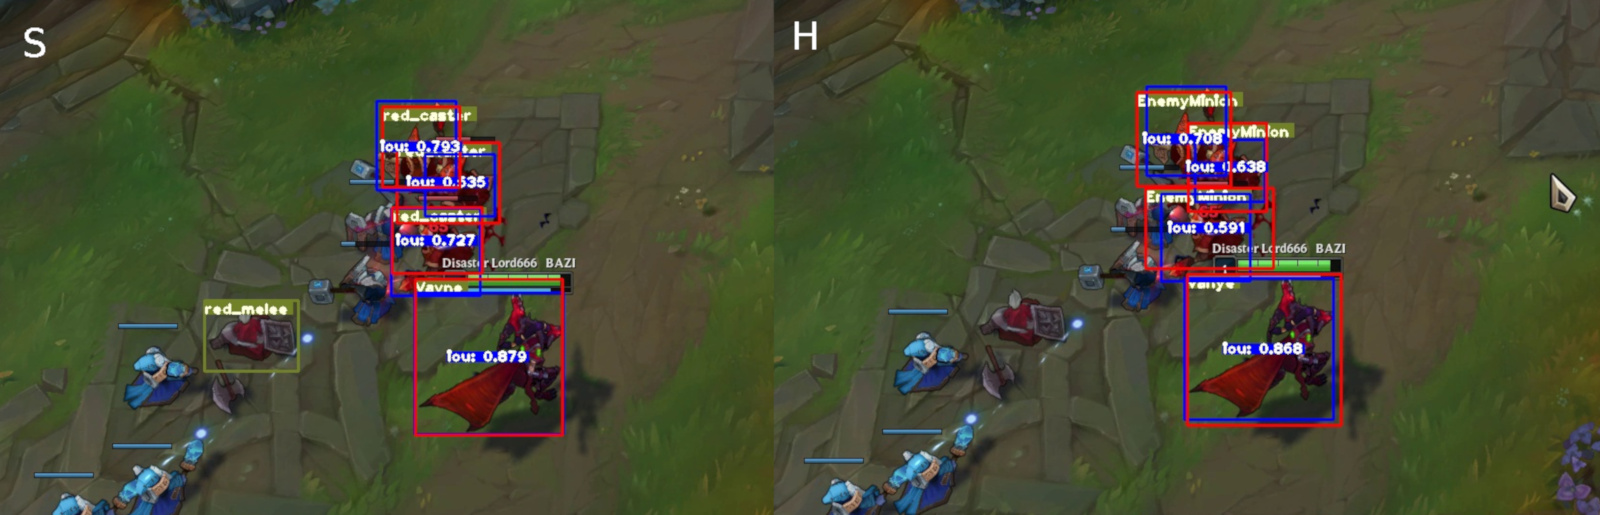
\includegraphics[width=\textwidth]{figures/new_wrong.jpg}
\caption{Model $\mathcal{S}$ detects dead minions. While this shows the better performance of $\mathcal{S}$, this is a problem that needs to be addressed in the future.}
\label{fig:new_wrong}
\end{figure*}

In Figure \ref{fig:new_wrong} both models detected all objects correctly, we can see that $\mathcal{S}$ detected in addition a melee minion that had already died.
Dead minions were not part of the synthetic training data, indicating that the model is capable of generalizing to unseen data.
The synthetic data takes more perspectives of all the objects and introduces noise and is thus able to better generalize to unseen objects.
On the other hand detecting dead minions is not a desired behavior of the object detector and thus in the future it could help to add dead minions as negative examples to the training dataset in order to prevent these missdetections.
\begin{figure*}
\centering
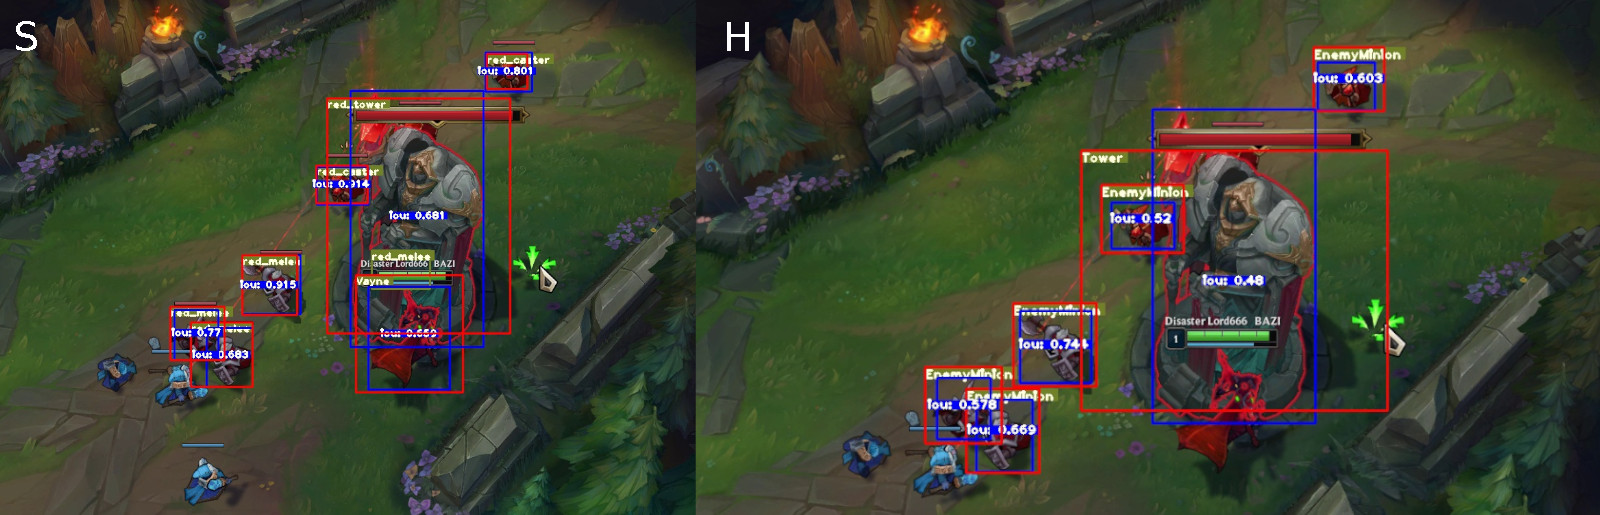
\includegraphics[width=\textwidth]{figures/new_better.jpg}
\caption{Model $\mathcal{S}$ is capable of handling overlapping objects better.}
\label{fig:new_better}
\end{figure*}

Figure \ref{fig:new_better} shows an example where model $\mathcal{S}$ clearly outperforms $\mathcal{H}$.
We can see that on the left side the predicted bounding boxes match the ground truth better and the IoU ratios are higher.
Furthermore, model $\mathcal{H}$ was not able to detect the player character which was overlapping the tower.
In the game this would lead to a dangerous loss of tracking next to a dangerous map objective such as an enemy tower.
We can see that $\mathcal{S}$ is better able to handle overlapping objects.
\begin{figure*}
\centering
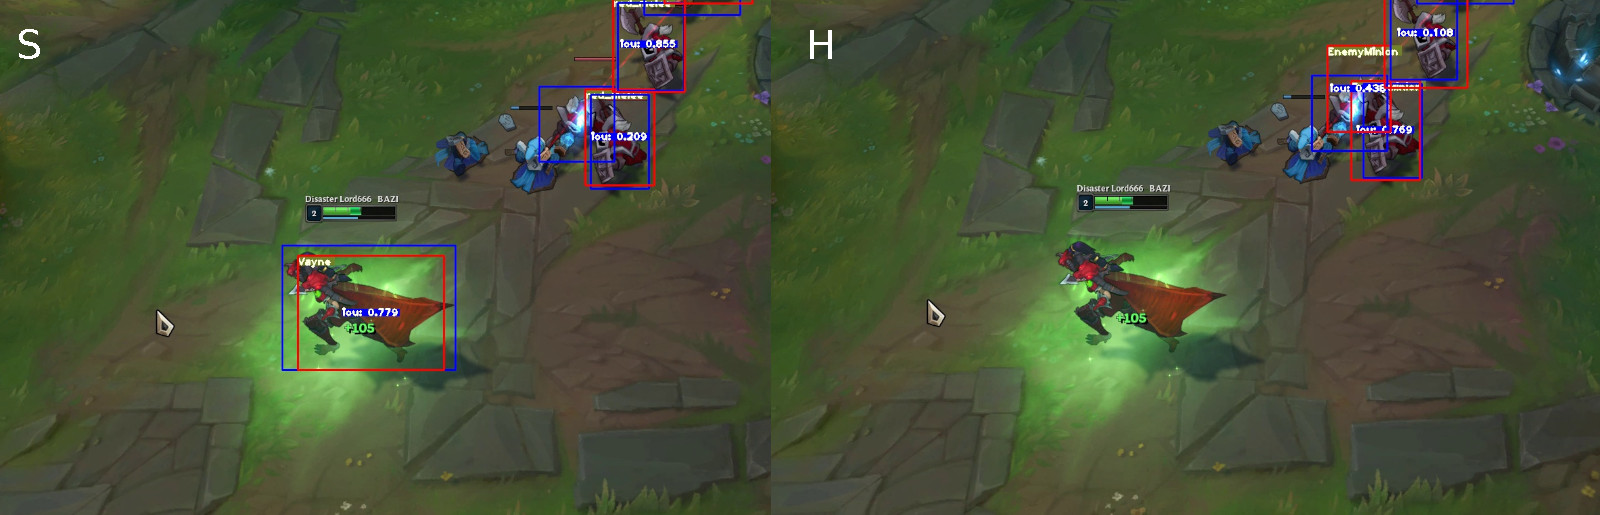
\includegraphics[width=\textwidth]{figures/new_better2.jpg}
\caption{Model $\mathcal{S}$ is better able to generalize and can still detect the player character while using abilities that add additional particles.}
\label{fig:new_better2}
\end{figure*}
In Figure \ref{fig:new_better2} we can see another example for the increased flexibility of model $\mathcal{S}$.
In this situation the player character used a spell which leads to the display of additional green particles around and on top of the character.
We can see that $\mathcal{S}$ was still capable of detecting the champion.
This is most likely a result of the introduced blur and noise as well as the larger amount of training data, allowing $\mathcal{S}$ to better handle the additional color changes.

\subsection{Combining the datasets}
In order to confirm the findings in \cite{rajpura2017object} and \cite{prakash2018structured}, that combining hand labeled and synthetic data can improve the performance of object detectors, both the datasets from $\mathcal{S}$ and $\mathcal{H}$ have been combined and used to train a model $\mathcal{C}$.
As can be seen in Table \ref{tab:2} the performance of $\mathcal{C}$ was in between $\mathcal{S}$ and $\mathcal{H}$.
In the video comparison the combined model actually performs worse than the other models, with most of the errors being cause by not detecting the player character.
This does not match the expectations as more different hand labeled data should at least provide similar performance to the synthetic data.
The reason for this is most likely the different aspect ratio of the synthetic and hand labeled images.
Furthermore, I had to reduce the number of classes in the synthetic dataset to 3 by combining all minion types into one.
Therefore, retraining the combined model with similar data is very likely going to further improve the performance.
In the future I will probably create a new hand labeled dataset for the minions of both teams, because Figure \ref{fig:results_old} and \ref{fig:results_new} as well as Table \ref{tab:2} show that the detection on the minions is the most unprecise and could therefore benefit from additional human labeled data.
Additionally hand labeled data on these smaller, often overlapping and more frequent occurring objects might improve detection quality.

